\chapter{Architektur}
Die folgenden UML-Diagramme sind nicht vollständig.
Wir versuchen einen kleinen aber dennoch guten Einblick in unsere Architektur zu liefern.
Dieser Abschnitt sicher spannend für technikinteressierte Leser. Man muss jedoch kein Informatiker sein, um dieses Kapitel zu verstehen.

\section{Klassendiagramm}
Folgend ist der Klassenaufbau unseres Spieles zu sehen.
Das rote (S) steht für Singleton.
Dies sind Klassen, die im ganzen Spiel nur genau einmal existieren können.
Die erste Graphik zeigt den momentanen Stand, wobei mit der Entwicklung des Deckbauers die neue Klasse "DeckManager" hinzukommen wird. \\
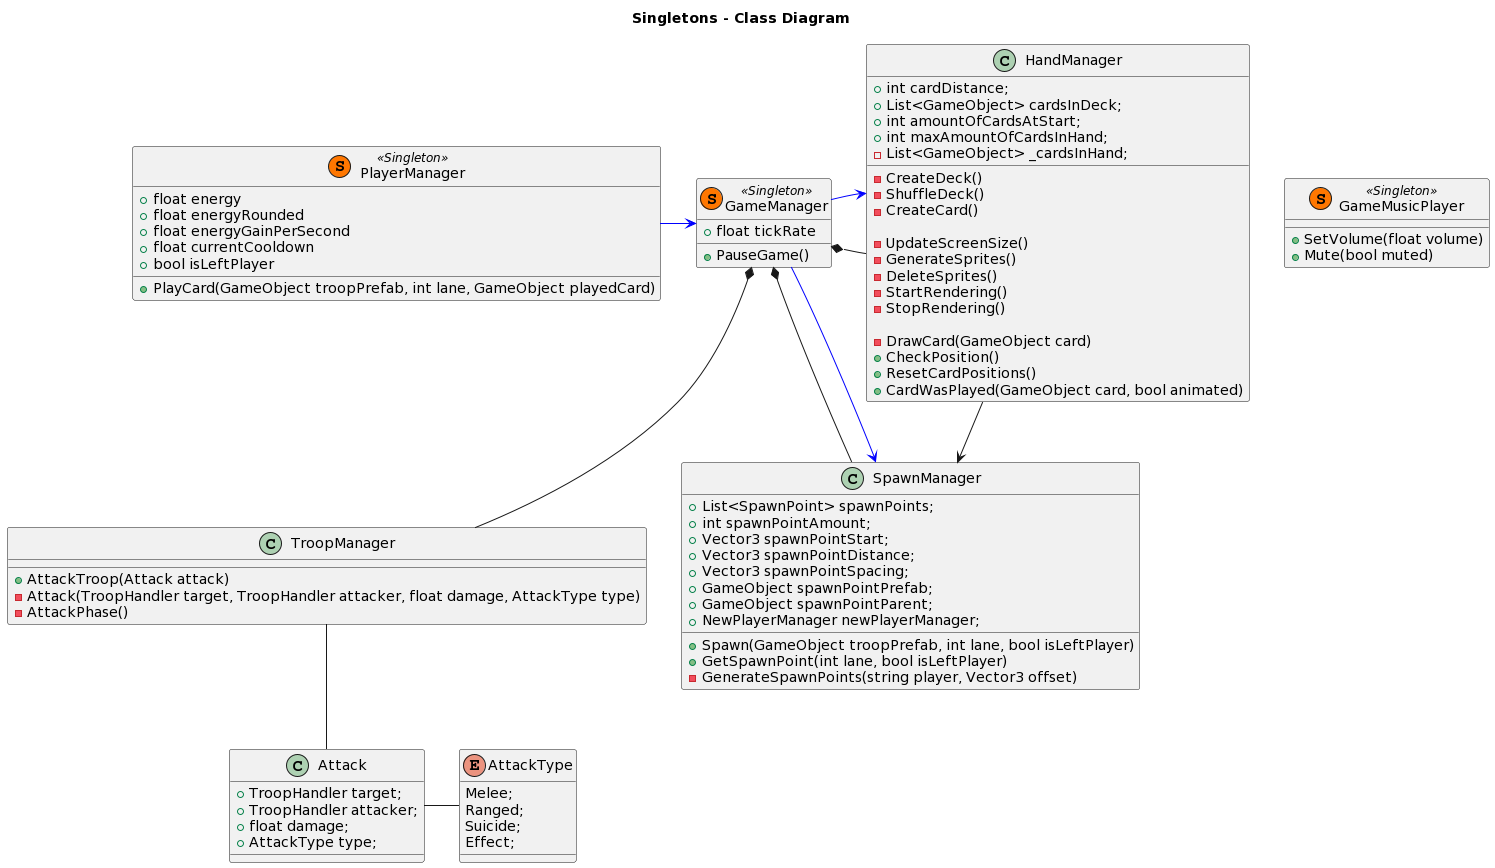
\includegraphics[width=14cm]{resources/Singletons.png} \\
\textit{momentaner Aufbau} \\
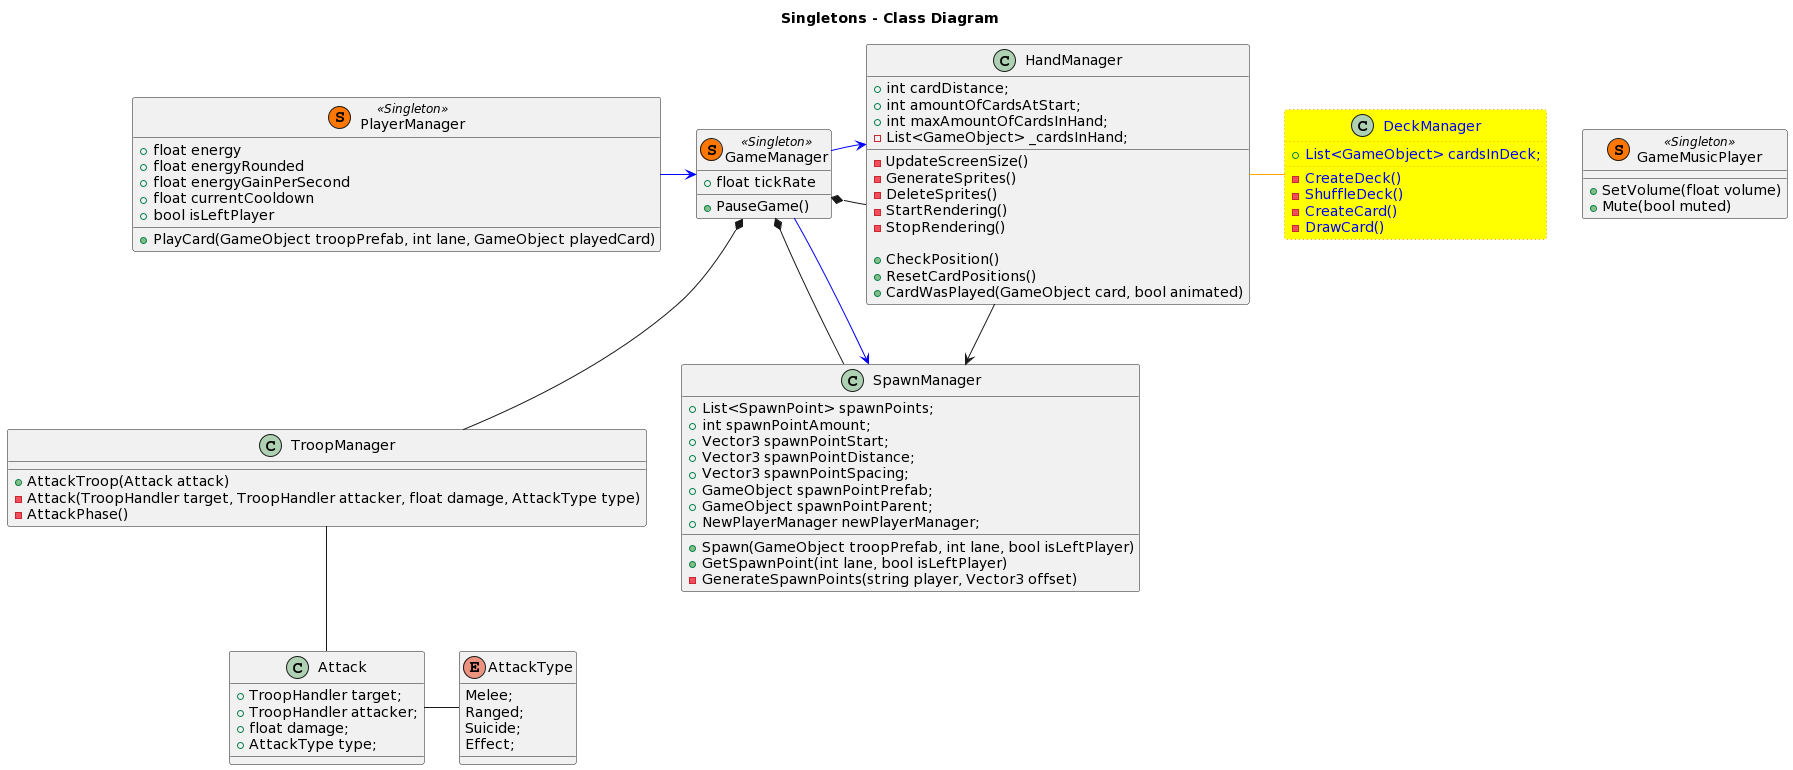
\includegraphics[width=14.5cm]{resources/Singletons 2.png} \\
\textit{zukünftiger Aufbau}

\section{Sequenzdiagramme}
\subsection{Nahkampftruppe}
Folgend ist die Abfolge unseres Codes zusehen, falls eine Truppe in Reichweite einer Nahkampftruppe kommt.\\
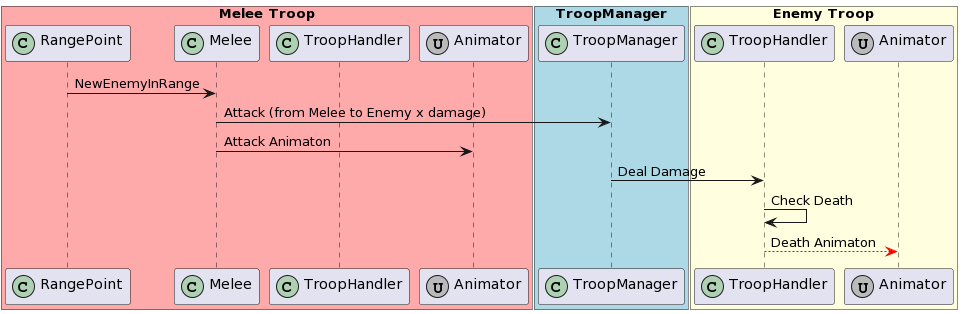
\includegraphics[width=15cm]{resources/MeleeAttacks.png} \\
\subsection{Suizidtruppe}
Da die Suizidtruppe auf den gleichen Prinzipen basiert, ist sie hier mit der zweiten Abbildung abgebildet. \\
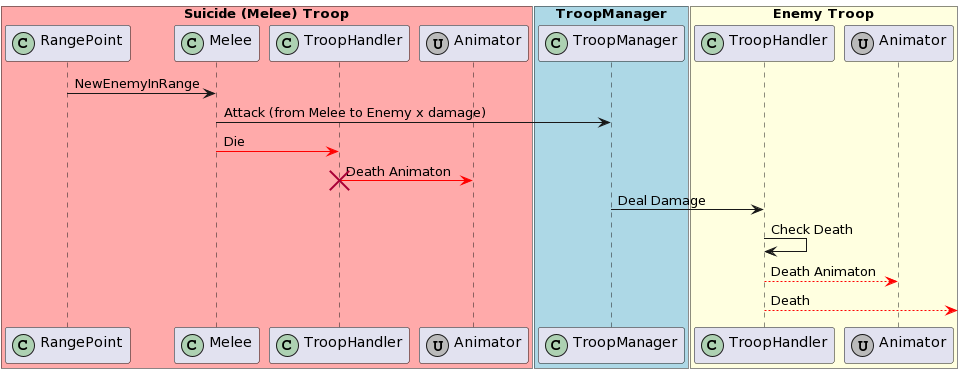
\includegraphics[width=15cm]{resources/SuicideAttacks.png} \\

\subsection{Fernkampftruppe}
Folgend ist abgebildet wie eine Fernkampftruppe auf einen neuen Gegner reagiert.\\
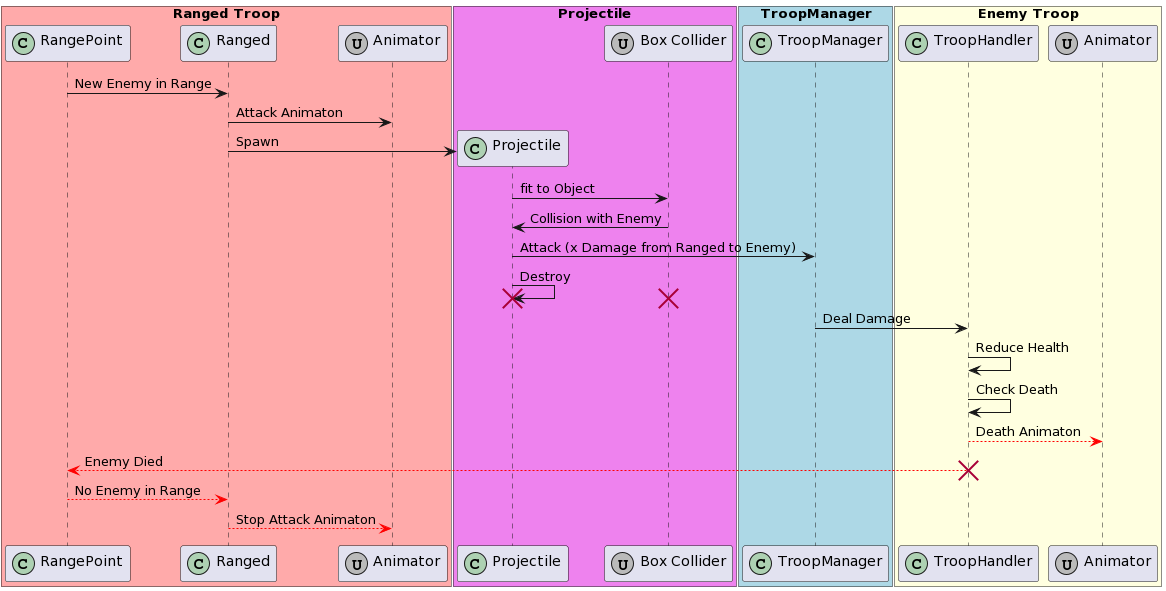
\includegraphics[width=15cm]{resources/RangedAttacks.png} \\
\\
Die folgende Abbildung zeigt den Ablauf, falls der Gegner stirbt und das Projektil keinen Schaden anrichtet\\
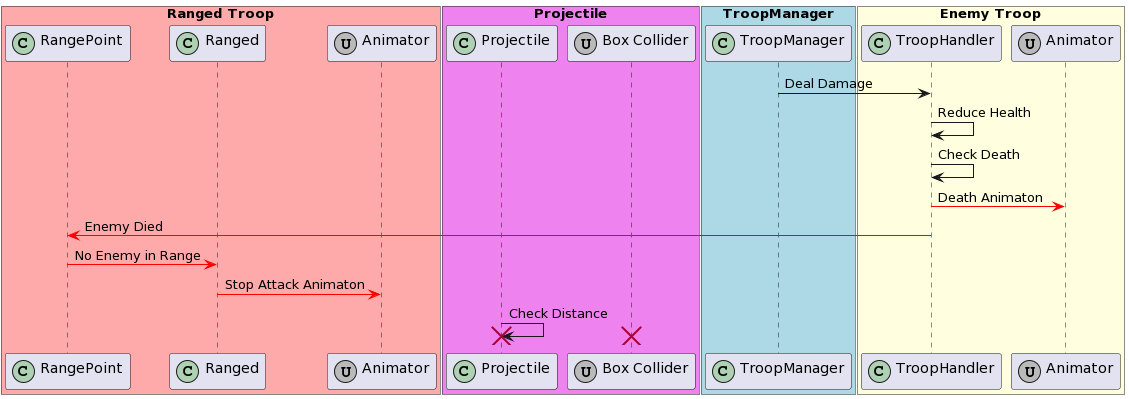
\includegraphics[width=15cm]{resources/Projectile.png}

\section{Gift}
Folgend ist die Sequenz abgebildet, falls eine giftige Truppe angegriffen wird. \\
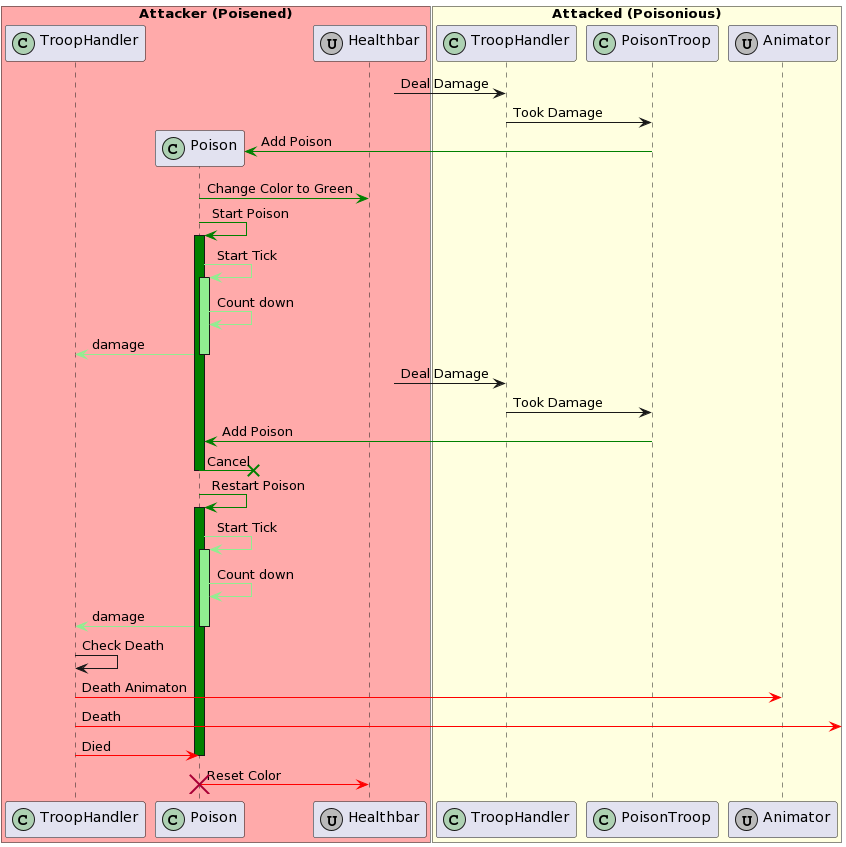
\includegraphics[width=15cm]{resources/Poison.png} \\


\section*{github file system / source / version control}
\url{https://www.youtube.com/watch?v=IQT37uwpcg4}